\section{Results and Discussion}\label{sec:results}
% P:results-01
The comparisons connect thermodynamic driving force, liquid-film resistance, and numerical solution cost to capture and axial temperature.
Thermodynamic model differences are examined first, followed by parameter sensitivity within the selected ePC-SAFT description.
The film and numerical comparisons then establish the effects of the transfer treatment and the effort required to resolve the coupled equations.
The operating-condition study brings these responses together over the local Latin hypercube design.
Capture and temperature differences are interpreted alongside their mesh and quadrature refinement changes; the detailed accuracy and cost comparison is given in \cref{subsec:results-solvers}.

\subsection{Thermodynamic closure and absorber response}\label{subsec:results-thermodynamics}
\subsubsection{Capture across the operating cases}
% P:results-02
\Cref{fig:thermo-capture} compares the Henry-law, eNRTL, and ePC-SAFT capture predictions with the same experimental observations.
The parity representation shows the scale of agreement across cases, while signed casewise errors distinguish overprediction from underprediction.
The common-property comparison evaluates the thermodynamic descriptions without simultaneous changes in hydraulic or caloric inputs.
Where species or reaction parameters differ, the capture difference represents the combined thermodynamic-model effect defined in \cref{sec:methods}.

% CHECKLIST-BEGIN: finding-isothermal-control
% P:results-isothermal-control
The constructed isothermal control isolates a thermodynamic-package difference under common conventional transport.
Calibrated eNRTL predicts \qty{96.7335}{\percent} capture, compared with \qty{98.8612}{\percent} for the Henry-law reference, a decrease of 2.1277 percentage points.
Changing the initial mesh from 17 to 33 points changes capture by less than $1.1\times10^{-8}$ percentage points in either arm.
The two-model difference therefore exceeds the observed mesh-refinement change for this control.
Its imposed temperature and constructed feeds define a model comparison rather than an experimental capture-error estimate.
% CHECKLIST-END: finding-isothermal-control

% CHECKLIST-BEGIN: finding-1
% P:results-03
\noindent\textit{[Quantitative comparison: capture MAE and signed bias for each thermodynamic closure; the largest and smallest casewise differences; the ordering supported by the common case set.]}
% CHECKLIST-END: finding-1

% P:results-04
An aggregate error combines operating points with different gas-to-liquid ratios and lean loadings.
The casewise comparison therefore relates each model difference to its corresponding inlet conditions.
In particular, a difference at a high-capture condition is interpreted together with the residual outlet CO$_2$ flow, because a small percentage-point change can represent a substantial relative change in that remaining flow.

\begin{figure}[pos=htbp]
\centering
\fbox{\begin{minipage}[c][48mm][c]{0.93\linewidth}\centering
\textbf{Thermodynamic closure: capture comparison}\\[8mm]
\small (a) Predicted versus measured capture\\[3mm](b) Signed capture error by case
\end{minipage}}
% P:results-05
\caption{Henry-law, eNRTL, and ePC-SAFT capture comparisons under common density, caloric, transport, and hydraulic descriptions.
The parity line denotes equality with observation; the casewise panel uses capture-error units of percentage points.}
\label{fig:thermo-capture}
\end{figure}
% Replace the framed panel with the final figure; keep this label and update the caption to its exact case set.

\subsubsection{Speciation and fugacity along the column}
% P:results-06
The axial comparison in \cref{fig:thermo-profiles} relates the capture differences to molecular CO$_2$ availability, reactive species distribution, and interfacial driving force.
The apparent loading identifies the conserved CO$_2$ content, while the molecular CO$_2$ concentration and fugacity identify its local thermodynamic availability for transfer.
Separating these quantities is especially useful when two models predict similar overall loading but different distributions between dissolved molecular CO$_2$, carbamate, and bicarbonate.

% CHECKLIST-BEGIN: finding-2
% P:results-07
\noindent\textit{[Principal finding: the axial regions and species responsible for the thermodynamic difference, with the corresponding fugacity and loading changes.]}
% CHECKLIST-END: finding-2

% P:results-08
The gas and liquid fugacity profiles locate the regions of large and small driving force.
The cumulative uptake links these local differences to the integral capture in \cref{fig:thermo-capture}.
A change near the liquid inlet can alter the terminal approach to equilibrium, whereas a change over a broad section of the bed can redistribute absorption and the associated heat release.
The interpretation uses the local temperature and composition rather than attributing the entire column response to a single equilibrium-pressure value.

\begin{figure}[pos=htbp]
\centering
\fbox{\begin{minipage}[c][58mm][c]{0.93\linewidth}\centering
\textbf{Thermodynamic closure: axial state}\\[8mm]
\small (a) Apparent loading and molecular CO$_2$\\[3mm](b) Carbamate/bicarbonate distribution\\[3mm](c) Gas and liquid CO$_2$ fugacities
\end{minipage}}
% P:results-09
\caption{Matched axial profiles for the thermodynamic comparison.
The coordinate increases from the gas inlet to the liquid inlet.
Apparent loading, true-species quantities, and fugacity are reported on their respective defined bases.}
\label{fig:thermo-profiles}
\end{figure}
% Replace the framed panel with the final figure; keep this label and update the caption to its exact case set.

% P:results-isothermal-profiles
The control profiles in \cref{fig:isothermal-control} show more CO$_2$ remaining in the vapor with eNRTL over the bed and a lower rich-liquid loading at the gas inlet.
Both liquid profiles reach the same lean-feed loading at the top of the column.
These profiles connect the integral capture difference to the axial component balance under the imposed isothermal conditions.

\begin{figure}[pos=htbp]
\centering
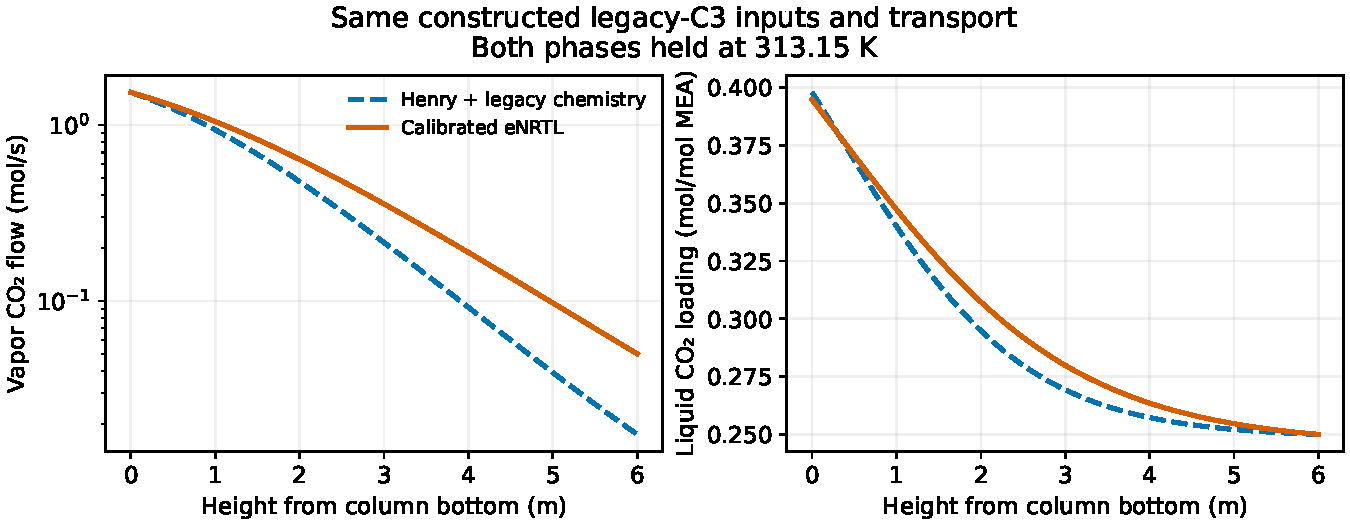
\includegraphics[width=\linewidth]{figures/isothermal-henry-enrtl-profiles.pdf}
% P:results-isothermal-caption
\caption{Calculated vapor CO$_2$ flow and apparent liquid loading for the constructed C3 isothermal control at \qty{313.15}{K}.
The Henry-law reference retains its conventional reaction description, whereas the eNRTL arm uses the calibrated six-species model; both use the same feeds and conventional transport.
The vapor-flow axis is logarithmic, and height increases from the gas inlet.
Profiles use the solutions initialized with 33 axial points.}
\label{fig:isothermal-control}
\end{figure}

\subsubsection{Density and caloric effects}
% P:results-10
\Cref{fig:full-property} extends the equilibrium comparison to the consistent density and enthalpy response of the selected thermodynamic description.
For any reported quantity $Q$, the paired changes can be written
\begin{align}
\Delta Q_{\mathrm{eq}}&=Q_{\mathrm{common},m}-Q_{\mathrm{common},\mathrm{ref}},\\
\Delta Q_{\mathrm{prop}}&=Q_{\mathrm{full},m}-Q_{\mathrm{common},m}.
\end{align}
Here $m$ denotes the thermodynamic model and the reference denotes the common-property comparison basis.
These paired changes follow the specified sequence of model substitutions.
They distinguish the equilibrium comparison from its additional volume and energy response, conditional on the retained transport model; a different substitution order can assign interacting effects differently.

% CHECKLIST-BEGIN: finding-3
% P:results-11
\noindent\textit{[Quantitative comparison: additional capture change, temperature-maximum change and axial shift, and temperature-tap RMSE for the full-property calculation.]}
% CHECKLIST-END: finding-3

% P:results-12
Density changes affect volumetric flow, velocity, holdup, and transfer coefficients.
Caloric changes alter the temperature response to the same local absorption and water transfer.
Because temperature feeds back into equilibrium and mobility, the full-property effect is interpreted through the coupled profiles rather than by adding isolated property errors.
The paired simulations retain the same feeds and packing specification throughout this comparison.

\begin{figure}[pos=htbp]
\centering
\fbox{\begin{minipage}[c][55mm][c]{0.93\linewidth}\centering
\textbf{Equilibrium and full-property effects}\\[8mm]
\small (a) Paired changes in capture\\[3mm](b) Liquid temperature and volumetric flow\\[3mm](c) Enthalpy and absorption distribution
\end{minipage}}
% P:results-13
\caption{Comparison of common-property and full-property calculations at matched operating conditions.
The panels separate the initial equilibrium/fugacity change from the additional density and caloric response.}
\label{fig:full-property}
\end{figure}
% Replace the framed panel with the final figure; keep this label and update the caption to its exact case set.

\subsection{Thermodynamic parameter sensitivity}\label{subsec:results-sensitivity}
% P:results-sensitivity-01
The preceding model comparison changes the thermodynamic description; the sensitivity comparison varies four parameter coordinates within the selected ePC-SAFT description at the Case 3C reference conditions.
The perturbation definitions are given in \cref{subsec:sensitivity-design}.
\Cref{fig:thermodynamic-sensitivity} distinguishes the locally recomputed driving force from the response after the complete column is resolved.
The local comparison retains analytical flows and temperature, while the coupled comparison allows absorption and heat release to redistribute along the bed.
A change in local fugacity therefore need not produce a proportional change in capture.

% CHECKLIST-BEGIN: finding-10
% P:results-sensitivity-02
\textit{[Thermodynamic sensitivity: signed capture and temperature changes for each prescribed perturbation, local and coupled fugacity/flux responses, and their size relative to numerical refinement.]}
% CHECKLIST-END: finding-10

\begin{figure}[pos=htbp]
\centering
\fbox{\begin{minipage}[c][48mm][c]{0.93\linewidth}\centering
\textbf{Case 3C thermodynamic sensitivity}\\[8mm]
\small (a) Signed capture and temperature changes\\[3mm](b) Local and coupled driving-force response
\end{minipage}}
\caption{Response to the two reaction-enthalpy directions, water solvation factor, and CO$_2$ dispersion energy at the Case 3C reference inputs. The positive and negative perturbations use the ranges in \cref{tab:operating-sensitivity-inputs}; capture changes are in percentage points and temperature changes in kelvin.}
\label{fig:thermodynamic-sensitivity}
\end{figure}

\subsection{Enhancement-factor and reactive-film transport}\label{subsec:results-film}
% P:results-film-transition
The thermodynamic comparisons describe the availability of CO$_2$ for transfer.
The film comparison examines how the liquid resistance converts that driving force into uptake at the same thermodynamic model and feed conditions.
\subsubsection{Capture and local transfer resistance}
% P:results-14
\Cref{fig:film-capture} compares the enhancement-factor and equilibrium-manifold transfer descriptions at common bulk thermodynamics.
The model difference is the representation of liquid-film resistance.
Both arms retain the same feed definitions, reaction equilibrium, gas-side resistance, water transfer, and packing correlations.
Their axial bulk states are independently calculated consequences of the selected film model.
The signed transfer-model effect for case $k$ is
\begin{align}
\Delta\eta_{k,\mathrm{film}}=\eta_{k,\mathrm{film}}-\eta_{k,\mathrm{enh}}.
\end{align}

% CHECKLIST-BEGIN: finding-4
% P:results-15
\noindent\textit{[Quantitative comparison: the range of capture changes, aggregate capture errors, and operating conditions associated with the largest transfer-model effect.]}
% CHECKLIST-END: finding-4

% P:results-16
The local interpretation follows the interfacial state and the integrated liquid resistance.
In the enhancement description, the Hatta number and finite reactant supply determine the effective liquid-film contribution.
In the equilibrium-manifold description, the reactive chemical-potential tangent and constrained mobility determine that contribution along the complete bulk-to-interface path.
These representations can be compared through their resulting fluxes without assigning the film calculation an empirical enhancement multiplier.

\begin{figure}[pos=htbp]
\centering
\fbox{\begin{minipage}[c][55mm][c]{0.93\linewidth}\centering
\textbf{Transfer-model comparison}\\[8mm]
\small (a) Enhancement and reactive-film capture\\[3mm](b) Casewise capture change\\[3mm](c) Local gas- and liquid-film resistance
\end{minipage}}
% P:results-17
\caption{Enhancement-factor and equilibrium-manifold film comparisons with the same thermodynamic model and feed conditions.
Each arm solves its own axial bulk states.
Positive capture change denotes greater uptake for the equilibrium-manifold calculation.}
\label{fig:film-capture}
\end{figure}
% Replace the framed panel with the final figure; keep this label and update the caption to its exact case set.

\subsubsection{Interfacial state and axial absorption}
% P:results-18
\Cref{fig:film-profiles} follows the local CO$_2$ flux, interfacial fugacity, and cumulative uptake along the bed.
The interface-root solution partitions the total driving force between gas and liquid resistances.
This partition connects a change in the local film law to the axial region in which the column response changes.
The cumulative uptake in \cref{eq:integral-uptake} then relates the local comparison to the total capture.

% CHECKLIST-BEGIN: finding-5
% P:results-19
\noindent\textit{[Principal finding: the dominant resistance, the axial region of the largest flux change, and the resulting redistribution of cumulative uptake.]}
% CHECKLIST-END: finding-5

% P:results-20
The film comparison also distinguishes a higher total uptake from a different distribution of uptake.
Two calculations can have similar outlet capture while locating absorption and heat release differently within the bed.
The interfacial and temperature profiles are therefore interpreted together with the integrated performance.
The water-transfer contribution is retained in the energy balance even though the CO$_2$ mobility calculation constrains its own water-component flux.

\begin{figure}[pos=htbp]
\centering
\fbox{\begin{minipage}[c][55mm][c]{0.93\linewidth}\centering
\textbf{Transfer-model comparison: axial response}\\[8mm]
\small (a) CO$_2$ flux and interfacial fugacity\\[3mm](b) Cumulative absorbed CO$_2$\\[3mm](c) Liquid and gas temperature
\end{minipage}}
% P:results-21
\caption{Axial transfer and temperature profiles for the enhancement-factor and equilibrium-manifold calculations.
Local fluxes integrate to the inlet/outlet material balance; cumulative uptake distinguishes total capture from its spatial distribution.}
\label{fig:film-profiles}
\end{figure}
% Replace the framed panel with the final figure; keep this label and update the caption to its exact case set.

\subsubsection{Mobility and film-thickness sensitivity}
% P:results-film-sensitivity-intro
\Cref{fig:film-sensitivity} relates changes in capture and temperature to species-group mobility and film thickness.
The separate perturbations defined in \cref{subsec:film-sensitivity-design} identify which transport inputs most influence the comparison with the enhancement-factor model.

% CHECKLIST-BEGIN: finding-6
% P:results-24
\noindent\textit{[Sensitivity findings: the influential mobility inputs, the selected perturbation ranges, the capture and temperature changes, and the persistence of the transfer-model comparison over those ranges.]}
% CHECKLIST-END: finding-6

% P:results-25
The mobility approximation represents species transport, while the equilibrium tangent represents thermodynamic response.
Keeping these contributions separate identifies whether a model difference is controlled mainly by the reaction-equilibrium path or by the assumed transport scale.
The sensitivity range follows the parameter sources and the stated physical assumptions, rather than a fit to the column capture observations.

\begin{figure}[pos=htbp]
\centering
\fbox{\begin{minipage}[c][48mm][c]{0.93\linewidth}\centering
\textbf{Film-input sensitivity}\\[8mm]
\small (a) Capture response to diffusivity groups\\[3mm](b) Capture and temperature response to film thickness
\end{minipage}}
% P:results-26
\caption{Sensitivity of the equilibrium-manifold calculation to the specified species diffusivities and physical film thickness.
Thermodynamic parameters and case inputs are held fixed.}
\label{fig:film-sensitivity}
\end{figure}
% Replace the framed panel with the final figure; keep this label and update the caption to its exact case set.

\subsection{Boundary-value solution methods}\label{subsec:results-solvers}
\subsubsection{Solution agreement and refinement}
% P:results-27
\Cref{fig:solver-accuracy} compares the conservative simultaneous formulation with shooting, finite differences, and collocation on identical physical equations.
The comparison uses capture, liquid-temperature profiles, and the integral balances to relate the numerical solutions.
Refinement varies the axial resolution and film quadrature separately, preserving the physical inputs.
The profile comparison includes the temperature maximum and its location, which can be more sensitive to resolution than the integrated capture.

% CHECKLIST-BEGIN: numerical-node-verification
% P:results-node-verification
A local verification of the conservative formulation compares the assembled $19\times12$ Jacobian with a centered directional difference at a synthetic interior test state, using a step of $10^{-3}$ along the prescribed physical direction.
The maximum rowwise relative discrepancy is $2.05\times10^{-7}$; the liquid-film, gas-CO$_2$, water-transfer, and energy rows give $6.22\times10^{-9}$, $7.70\times10^{-9}$, $2.83\times10^{-9}$, and $1.89\times10^{-10}$, respectively.
Each discrepancy is scaled by the larger magnitude of the analytic and difference estimates, with a denominator floor of $10^{-12}$.
The test-state construction and implementation identity are supplied in the supplementary verification record.
This comparison verifies derivative assembly at the tested state; full-column solution agreement and refinement are assessed separately in \cref{fig:solver-accuracy}.
% CHECKLIST-END: numerical-node-verification

% CHECKLIST-BEGIN: finding-7
% P:results-28
\noindent\textit{[Numerical findings: agreement in capture and temperature, mesh and quadrature refinement changes, and material/energy/charge conservation at the reported settings.]}
% CHECKLIST-END: finding-7

% P:results-29
The methods represent the same countercurrent coupling differently.
Shooting resolves it through a boundary root around an initial-value integration; finite differences solve a nodal algebraic system; collocation uses a continuous polynomial representation with residual-based refinement; the conservative simultaneous formulation balances physical flow quantities directly between nodes.
The comparison therefore associates cost with a specified solution accuracy and operating point.
It does not combine different physical models in a numerical-method ranking.

\begin{figure}[pos=htbp]
\centering
\fbox{\begin{minipage}[c][55mm][c]{0.93\linewidth}\centering
\textbf{Boundary-value solution accuracy}\\[8mm]
\small (a) Cross-method axial profiles\\[3mm](b) Capture and temperature changes with refinement\\[3mm](c) Integral material and energy balance
\end{minipage}}
% P:results-30
\caption{Solution agreement and refinement for conservative simultaneous, shooting, finite-difference, and collocation formulations applied to the same absorber equations.
Profile comparisons use common physical heights and the same inlet specification.}
\label{fig:solver-accuracy}
\end{figure}
% Replace the framed panel with the final figure; keep this label and update the caption to its exact case set.

% CHECKLIST-BEGIN: method-09
% P:methods-21
\Cref{tab:numerical-comparison} reports the accuracy and cost of each method at the same operating point and with the same physical equations.
Refinement changes are differences from the next finer calculation, while conservation errors are evaluated from the dimensional balances.

\begin{table}[pos=htbp]
\centering\small
\caption{Boundary-value method comparison at matched physical conditions. Capture refinement changes are in percentage points, temperature changes in kelvin, and runtime in seconds. The conservation column reports the scaled material, energy, and charge residuals.}
\label{tab:numerical-comparison}
\begin{tabularx}{\linewidth}{@{}lXXXXX@{}}
\toprule
Method & Nodes & $|\Delta\eta|$ & $\|\Delta T_l\|_\infty$ & Conservation & Runtime\\
\midrule
Shooting & \textit{[value]} & \textit{[value]} & \textit{[value]} & \textit{[values]} & \textit{[values]}\\
Finite differences & \textit{[value]} & \textit{[value]} & \textit{[value]} & \textit{[values]} & \textit{[values]}\\
Collocation & \textit{[value]} & \textit{[value]} & \textit{[value]} & \textit{[values]} & \textit{[values]}\\
Conservative simultaneous & \textit{[value]} & \textit{[value]} & \textit{[value]} & \textit{[values]} & \textit{[values]}\\
\bottomrule
\end{tabularx}
\end{table}
% CHECKLIST-END: method-09

\subsubsection{Computational cost}
% P:results-31
\Cref{fig:solver-cost} relates runtime to the achieved accuracy and identifies the contribution of local thermodynamics and film evaluation.
Repeated timings use the same hardware, thread configuration, and scope of calculation.
The timing comparison distinguishes a change in the number of local evaluations from a change in their individual cost.

% CHECKLIST-BEGIN: finding-8
% P:results-32
\noindent\textit{[Timing findings: median runtime and spread for each method, evaluation counts, final mesh sizes, and the operating-point dependence of the preferred method.]}
% CHECKLIST-END: finding-8

% P:results-33
A more expensive local thermodynamic model can change the balance between integration work and global nonlinear iterations.
The cost of the reactive film also depends on the quadrature resolution required along the equilibrium path.
The comparison is therefore interpreted jointly with the refinement results: the relevant computational saving is the reduction in time to obtain the same physical quantities to the same accuracy.

\begin{figure}[pos=htbp]
\centering
\fbox{\begin{minipage}[c][48mm][c]{0.93\linewidth}\centering
\textbf{Boundary-value solution cost}\\[8mm]
\small (a) Runtime versus achieved accuracy\\[3mm](b) Equilibrium, film, and column-solve contributions
\end{minipage}}
% P:results-34
\caption{Computational cost of the BVP formulations at matched numerical accuracy.
Timing scope, repeated-run summary, hardware, and thread configuration accompany the final comparison.}
\label{fig:solver-cost}
\end{figure}
% Replace the framed panel with the final figure; keep this label and update the caption to its exact case set.

\subsection{Operating-condition response}\label{subsec:results-operating}
% P:results-operating-01
\Cref{fig:operating-screen} relates the sampled operating conditions to capture, gas and liquid outlet temperatures, and the temperature maxima and their locations.
Gas throughput and liquid circulation are described on the mass basis defined in \cref{subsec:sensitivity-design}, while lean loading and MEA fraction determine the incoming solvent composition.
The thermodynamic and transport coordinates vary alongside these operating inputs, so response trends are interpreted jointly rather than assigned to a single operating variable from an unadjusted scatter plot.
The common diffusivity multiplier examines the overall mobility scale; it does not resolve relative uncertainty among individual ionic diffusivities.

% CHECKLIST-BEGIN: finding-11
% P:results-operating-02
\textit{[Operating-condition findings: sampled capture and temperature ranges, supported response directions and input rankings, additive-model prediction quality, and the operating tradeoffs supported within the sampled domain.]}
% CHECKLIST-END: finding-11

% P:results-operating-03
The operating comparison extends the reference-case sensitivity in \cref{subsec:results-sensitivity} to simultaneous changes in feeds, thermodynamic parameters, and transport properties.
Capture and the thermal response are considered jointly within the selected ranges.
Their comparison is conditional on the one-bed geometry, assumed inlet humidity and liquid temperature, and fixed gas temperature and pressure specification.
An operating point with higher capture may require greater solvent circulation or alter the temperature maximum; those consequences are retained in the comparison.
A plant-level optimum additionally depends on regeneration duty, hydraulic limits, and the selected economic or energy objective.

\begin{figure}[pos=htbp]
\centering
\fbox{\begin{minipage}[c][48mm][c]{0.93\linewidth}\centering
\textbf{Local operating-condition comparison}\\[8mm]
\small (a) Capture and thermal response across sampled conditions\\[3mm](b) Supported thermodynamic, transport, and operating effects
\end{minipage}}
\caption{Capture and temperature response for the 48-point Latin hypercube design around Case 3C. The input ranges are given in \cref{tab:operating-sensitivity-inputs}; the response panels use the sampled operating conditions, and the ranges are exploratory rather than probability intervals.}
\label{fig:operating-screen}
\end{figure}

\subsection{Integrated absorber response and engineering interpretation}\label{subsec:results-implications}
% P:results-35
The model comparisons and sensitivity studies connect the representation of the absorber to its operating response.
The thermodynamic comparison identifies the effect of equilibrium and property descriptions, while the parameter study identifies the inputs that control that response within ePC-SAFT.
The film comparison isolates the transfer treatment at common thermodynamics, and the numerical comparison quantifies the effort needed to resolve the same physical equations.
The Latin hypercube study examines how these dependencies influence capture and temperature over the specified operating neighborhood.

% CHECKLIST-BEGIN: finding-9
% P:results-36
\noindent\textit{[Cross-study synthesis: relative magnitude of thermodynamic, transfer, and numerical effects; the supported choice of model and solution method; the sensitivity and operating tradeoffs that qualify that choice; the capture and temperature evidence supporting the interpretation.]}
% CHECKLIST-END: finding-9

% P:results-37
The experimental temperature profile provides a spatial constraint on this interpretation.
Agreement in capture is accompanied by the position and magnitude of heat release, with water evaporation and interphase heat exchange represented in the same energy balance.
A comparison that improves one observable is assessed against its effect on the others.
The physical assumptions remain the local reaction-equilibrium approximation, the mobility description, nontransfer of MEA and gas inerts, the separate water-transfer law, and the parameter temperature domains.

% P:results-38
The scope is a one-bed absorber with specified feeds and packing.
Extensions to intercooling, substantial pressure drop, or additional volatile components require the corresponding material and energy terms.
The results of the controlled studies provide the basis for selecting which thermodynamic and transfer detail is needed for the operating range examined here.
